 ------------------------------------------------------------------------------
% Chapter 1
% ------------------------------------------------------------------------------
\chapter{Project} % enter the name of the section here
\section{ProjectIdea}
The project centers around the development of an application designed to function as a virtual therapist. The primary goal is to provide accessible and personalized mental health support in an increasingly fast-paced and interconnected world. The application utilizes artificial intelligence and machine learning to create an empathetic and intelligent virtual therapist capable of engaging with users in a meaningful way.

Key Features:

    Personalized Support: The virtual therapist is designed to offer tailored assistance, taking into account individual needs, preferences, and mental health concerns. Through advanced algorithms, the application adapts its responses to the user's specific emotional state and context.

    Confidential and Non-Judgmental Space: Recognizing the importance of privacy in mental health discussions, the application creates a secure and confidential environment. Users can freely express their thoughts and emotions without fear of judgment, fostering a sense of trust and openness.

    User-Friendly Interface: The project prioritizes a user-friendly interface to ensure that individuals, regardless of their technological proficiency, can easily navigate and interact with the virtual therapist. The goal is to make mental health support accessible to a broad audience.

    Integration of AI and Machine Learning: Leveraging the latest advancements in artificial intelligence and machine learning, the virtual therapist continuously learns and improves its responses over time. This dynamic adaptation ensures a more effective and personalized support system for users.

    Addressing Mental Health Stigma: The project aims to contribute to the destigmatization of mental health issues by providing a digital platform that encourages users to seek help in a discreet and comfortable manner.

Throughout the development process, ethical considerations are a key focus, ensuring user privacy, data security, and adherence to established mental health care guidelines. The project envisions making a meaningful impact on the mental well-being of individuals globally by offering a modern, technology-driven approach to mental health support.
 
\newpage
\section{Use Case}
\begin{figure}[h]
    \begin{center}
        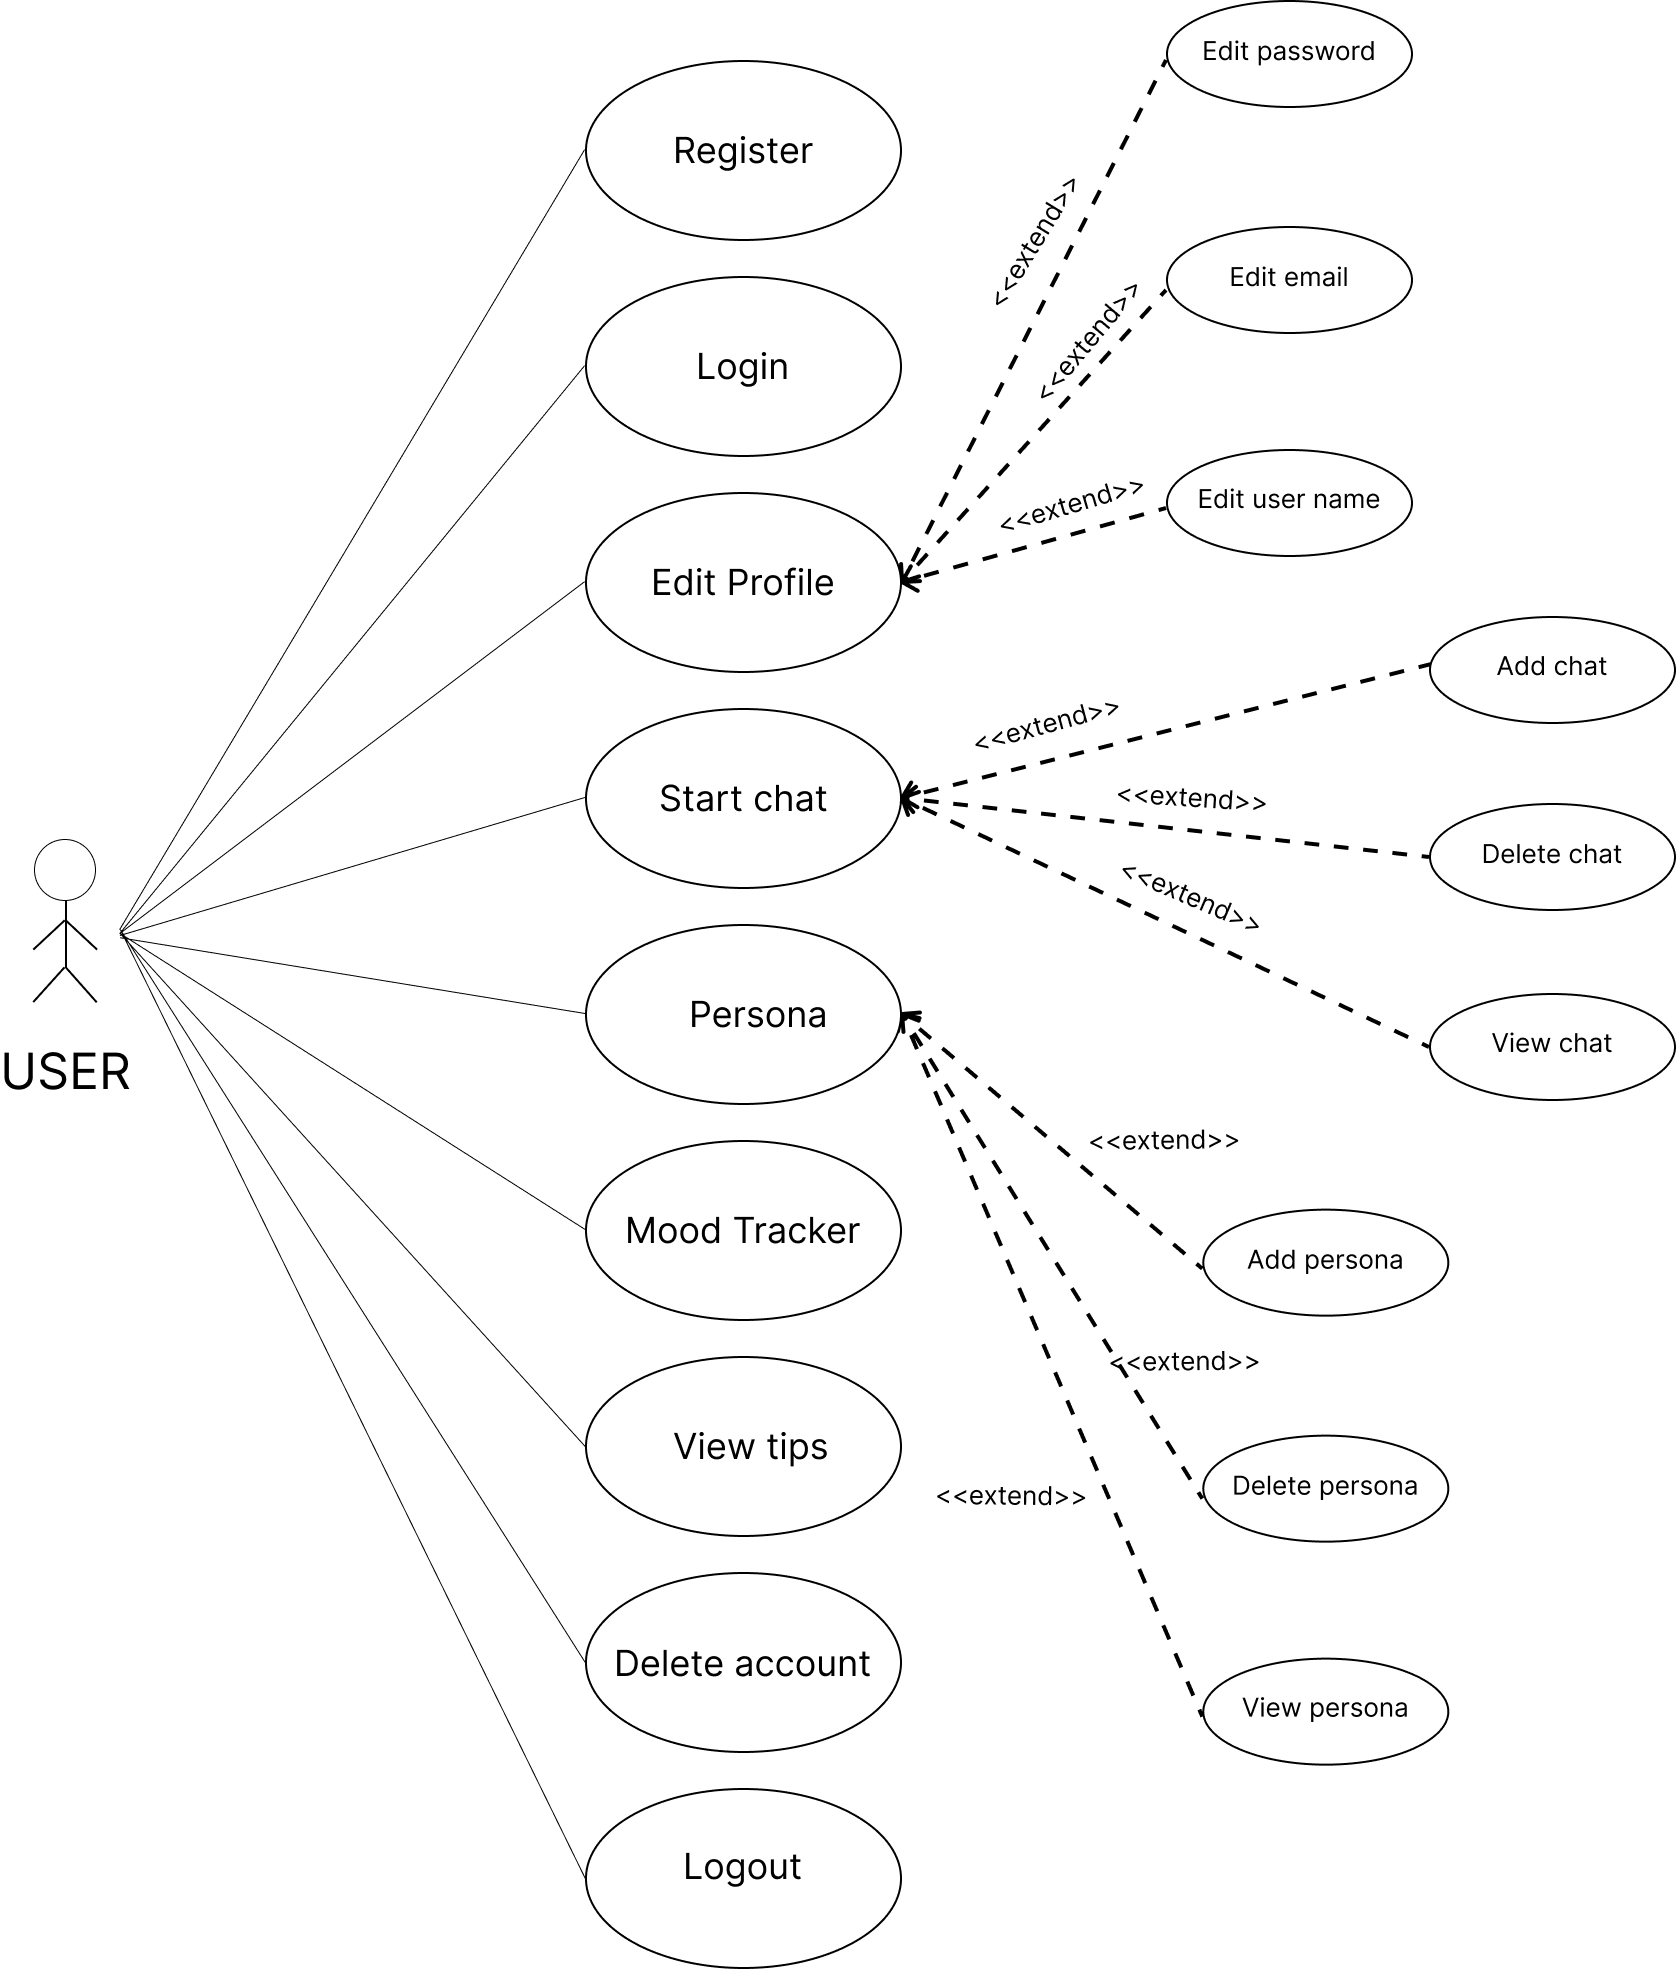
\includegraphics[width=5.5in]{uc}
    \end{center}
\centering
\end{figure}



\newpage
\section{TimeLine}
\begin{figure}[h]
    \begin{center}
        % 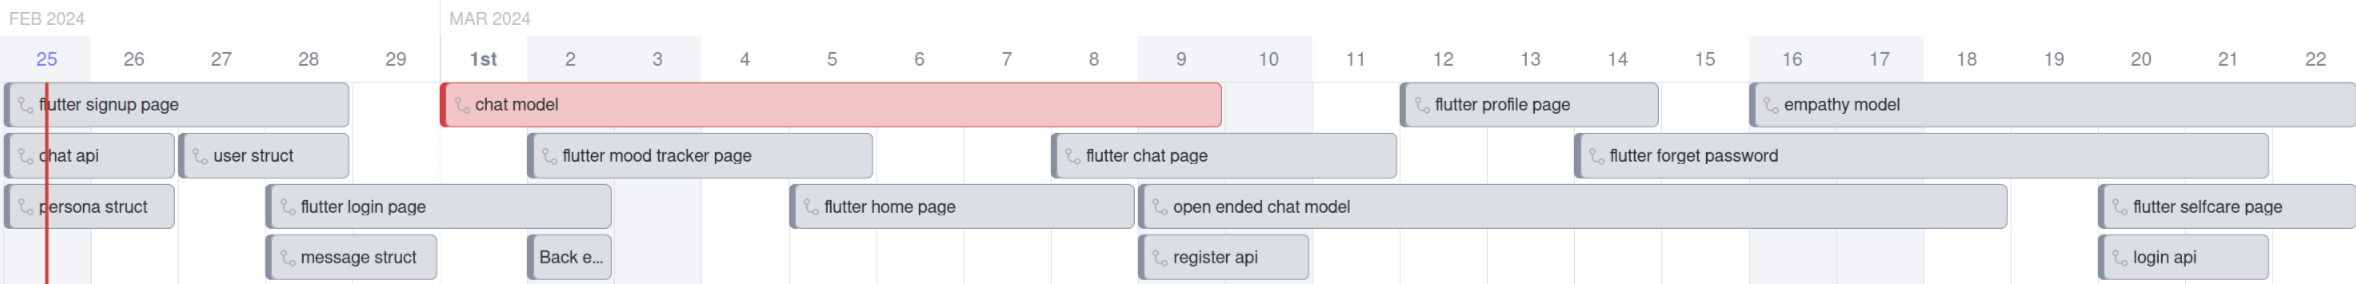
\includegraphics[width=7.0in]{timeline}
    \end{center}
\centering
\end{figure}
